\chapter{Variance of diffusion in $n$ dimensions} \label{sec:A5_variance}

The variance is a measurement of dispersion, comparing the standard deviation of a random variable to the population mean. The variance of function $f\qty(x)$ is defined as:

\begin{equation}
    \begin{aligned}
        \mathrm{Var}\qty(X)&=\sigma^2 \\
        &=E\qty(X^2)-E\qty(X)^2 \text{ ,} 
    \end{aligned}
\end{equation}
\noindent where $E\qty(X^n)$ is the expected value of variable $X^n$:
\begin{equation}
    \begin{aligned}
        E\qty(X^n)&=\int_{-\infty}^\infty x^nf\qty(x)\dd{x}\text{ .}
    \end{aligned}
\end{equation}
\par~\par 
The distance that cosmic rays have travelled via diffusion (see \autoref{chapter_1_cr_propagation} and \autoref{sec:09_Transport_multizone_diffusion}) can be approximated by the radius containing $1\sigma=68\%$ of the particles, $r_\sigma$. This Appendix will calculate the variance (therefore $r_\sigma$) for diffusion in 1D, 2D and 3D. 

\section{1D Diffusion}

\noindent For 1D isotropic diffusion, the solution to the transport equation for an impulsive accelerator injecting cosmic rays at $t=0$ and $x=0$ in a diffusion-only scenario (see \autoref{eq:chapter_7_cr_ev_green_solution}):

\begin{equation}
    \begin{aligned}
        n\qty(x)&=\frac{1}{\sqrt{4\pi Dt}}\exp(-\frac{x^2}{4Dt})\text{ .} 
    \end{aligned}
\end{equation}
\noindent Therefore:

\begin{equation}
    \begin{aligned}
        E\qty(x)&=\frac{1}{\sqrt{4\pi Dt}}\int_{-\infty}^\infty x\exp(-\frac{x^2}{4Dt})\dd{x} \\
        &=\frac{1}{\sqrt{4\pi Dt}}\qty(-2Dt\exp(-\frac{x^2}{4Dt})\bigg|_\infty+2Dt\exp(-\frac{x^2}{4Dt})\bigg|_{-\infty}) \\
        &=0\text{ ,} 
    \end{aligned}
\end{equation}
\noindent and:

\begin{equation}
    \begin{aligned}
        E\qty(x^2)&=\frac{1}{\sqrt{4\pi Dt}}\int_{-\infty}^\infty x^2\exp(-\frac{x^2}{4Dt})\dd{x} \\
        &=\frac{1}{\sqrt{4\pi Dt}} \qty(\frac{\pi^\frac{1}{2} \qty(4Dt)^\frac{3}{2}}{2}) \\
        &=2Dt\text{ .} 
    \end{aligned}
\end{equation}
\noindent This gives the variance in 1D:

\begin{equation}
    \begin{aligned}
        \mathrm{Var}\qty(x)&=2Dt\text{ ,} 
    \end{aligned}
\end{equation}
\noindent where $R_\sigma=\sqrt{2Dt}$ represents the radius containing $1\sigma\approx 68\%$ of cosmic rays.

\section{2D Diffusion}

For 2D diffusion, the solution to the transport equation for an impulsive accelerator injecting cosmic rays at $t=0$ and $r=0$ in a diffusion-only scenario (see \autoref{eq:chapter_7_cr_ev_green_solution}):

\begin{equation}
    \begin{aligned}
        n\qty(r)&=\frac{1}{4\pi Dt}\exp(-\frac{r^2}{4Dt}) \\
        r^2&=x^2+y^2\text{ .} 
    \end{aligned}
\end{equation}
For two variables $X$ and $Y$ with expected values $E\qty(X)$ and $E\qty(Y)$, the expected value of $X+Y$ is:

\begin{equation}
    \begin{aligned}
        E\qty(X+Y)&=E\qty(X)+E\qty(Y)\text{ .} 
    \end{aligned}
\end{equation}
\noindent Therefore, the expected value of $r^2$:

\begin{equation}
    \begin{aligned}
        E\qty(r^2)&=E\qty(x^2+y^2) \\
        &=E\qty(x^2)+E\qty(y^2) \\
        &= 2Dt + 2Dt \\
        &=4Dt\text{ .} 
    \end{aligned}
\end{equation}

\noindent The variance in 2D is:

\begin{equation}
    \begin{aligned}
        \mathrm{Var}\qty(r)&=4Dt\text{ .} 
    \end{aligned}
\end{equation}

\section{3D Diffusion}

For 3D diffusion, the solution to the transport equation for an impulsive accelerator injecting cosmic rays at $t=0$ and $r=0$ in a diffusion-only scenario (see \autoref{eq:chapter_7_cr_ev_green_solution}):

\begin{equation}
    \begin{aligned}
        n\qty(r)&=\frac{1}{\pi^{\frac{3}{2}} R_\text{diff}}\exp(-\frac{r^2}{R_\text{diff}^2}) \\
        R_\text{diff}&=\sqrt{4Dt}\text{ ,} 
    \end{aligned}
\end{equation}
\noindent where $r^2=x^2+y^2+z^2$. As with 2D diffusion:

\begin{equation}
    \begin{aligned}
        E\qty(r^2)&=E\qty(x^2)+E\qty(y^2)+E\qty(z^2) \\
        &= 2Dt + 2Dt + 2Dt \\
        &=6Dt\text{ .} 
    \end{aligned}
\end{equation}
\noindent The variance in 3D is:

\begin{equation}
    \begin{aligned}
        \mathrm{Var}\qty(r)&=6Dt\text{ .} 
    \end{aligned}
\end{equation}
\noindent The radius containing $1\sigma=68\%$ of cosmic rays $R_{\sigma}=\sqrt{\mathrm{Var}\qty(r)}=\sqrt{6Dt}$ does not equate to the `diffusion distance', $R_\text{diff}=\sqrt{4Dt}$, defined in literature (e.g. see \cite{1995PhRvD..52.3265A}) .
\par~\par 
Note that by taking a slice along the 3D energy distribution (e.g. $n(x,y,z=0)$), the radius ($r^2=x^2+y^2$) containing $68\%$ of cosmic rays reverts back to the 2D situation ($R_\sigma=\sqrt{4Dt}$). This can be seen in \autoref{fig:A4_multizone_diffusion_only}.

\begin{figure}[b!]
    \centering
    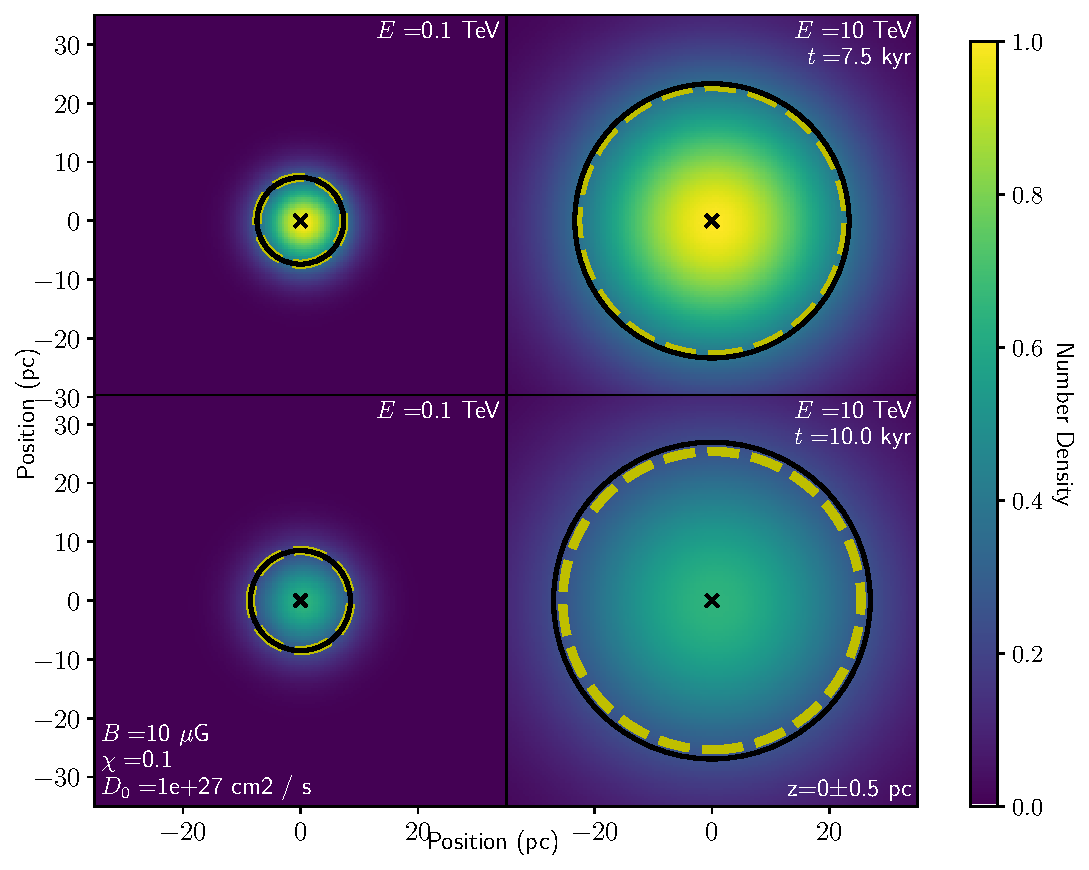
\includegraphics[width=0.9\textwidth]{A4_Variance_diffusion/Images/diffusion_3D.pdf}
    \begin{tabular}{c c c c c c}
      \toprule
      t (kyr) & E (TeV) & $R_\text{var}=\sqrt{4Dt}$ (pc) & $R_{\sigma\text{, 2D}}$ (pc) & $R_\text{var}=\sqrt{6Dt}$ (pc) & $R_{\sigma\text{, 3D}}$ (pc) \\
      \midrule
      5.0 & 0.1 & 6.0 & 6.0 & 7.4 & 7.4 \\
      $\sim$ & 10 & 19.1 & 19.0 & 23.3 & 23.3 \\
      10 & 0.1 & 8.5 & 8.5 & 10.4 & 10.4 \\
      $\sim$ & 10 & 26.9 & 25.4 & 33.0 & 31.1 \\
      \bottomrule
    \end{tabular}
    \caption{Evolution of the electron number density for a diffusion-only scenario taken at $z=0\pm 0.5~\pc$ along the line of sight. Electrons with energy $0.1~\TeV$ and $10~\TeV$ are injected at position $x=y=z=0$ (black cross) at $t=0$ into a uniform medium with magnetic field $B=10~\si{\micro G}$, $\chi=0.1$ and $D_0=10^{27}~\si{\centi\meter\squared\per\second}$ at $1~\GeV$. The electron number density is normalised to the maximum value in the 3D grid at $t=5.0~\kiloyear$. The black and yellow-dashed circles represents the 2D variance radius ($R_\text{var}=\sqrt{4Dt}$) and the radius $r_{\sigma\text{, 2D}}$ containing $68\%$ of electrons in the $z=0\pm 0.5~\pc$ slice. $R_\text{var}=\sqrt{6Dt}$ and $R_{\sigma\text{, 3D}}$ are the 3D variance radius and radius containing $68\%$ of electrons.}   \label{fig:A4_multizone_diffusion_only}
\end{figure}